\PassOptionsToPackage{unicode=true}{hyperref} % options for packages loaded elsewhere
\PassOptionsToPackage{hyphens}{url}
%
\documentclass[ignorenonframetext,]{beamer}
\usepackage{pgfpages}
\setbeamertemplate{caption}[numbered]
\setbeamertemplate{caption label separator}{: }
\setbeamercolor{caption name}{fg=normal text.fg}
\beamertemplatenavigationsymbolsempty
% Prevent slide breaks in the middle of a paragraph:
\widowpenalties 1 10000
\raggedbottom
\setbeamertemplate{part page}{
\centering
\begin{beamercolorbox}[sep=16pt,center]{part title}
  \usebeamerfont{part title}\insertpart\par
\end{beamercolorbox}
}
\setbeamertemplate{section page}{
\centering
\begin{beamercolorbox}[sep=12pt,center]{part title}
  \usebeamerfont{section title}\insertsection\par
\end{beamercolorbox}
}
\setbeamertemplate{subsection page}{
\centering
\begin{beamercolorbox}[sep=8pt,center]{part title}
  \usebeamerfont{subsection title}\insertsubsection\par
\end{beamercolorbox}
}
\AtBeginPart{
  \frame{\partpage}
}
\AtBeginSection{
  \ifbibliography
  \else
    \frame{\sectionpage}
  \fi
}
\AtBeginSubsection{
  \frame{\subsectionpage}
}
\usepackage{lmodern}
\usepackage{amssymb,amsmath}
\usepackage{ifxetex,ifluatex}
\usepackage{fixltx2e} % provides \textsubscript
\ifnum 0\ifxetex 1\fi\ifluatex 1\fi=0 % if pdftex
  \usepackage[T1]{fontenc}
  \usepackage[utf8]{inputenc}
  \usepackage{textcomp} % provides euro and other symbols
\else % if luatex or xelatex
  \usepackage{unicode-math}
  \defaultfontfeatures{Ligatures=TeX,Scale=MatchLowercase}
\fi
\usetheme[]{metropolis}
% use upquote if available, for straight quotes in verbatim environments
\IfFileExists{upquote.sty}{\usepackage{upquote}}{}
% use microtype if available
\IfFileExists{microtype.sty}{%
\usepackage[]{microtype}
\UseMicrotypeSet[protrusion]{basicmath} % disable protrusion for tt fonts
}{}
\IfFileExists{parskip.sty}{%
\usepackage{parskip}
}{% else
\setlength{\parindent}{0pt}
\setlength{\parskip}{6pt plus 2pt minus 1pt}
}
\usepackage{hyperref}
\hypersetup{
            pdfborder={0 0 0},
            breaklinks=true}
\urlstyle{same}  % don't use monospace font for urls
\newif\ifbibliography
\usepackage{graphicx,grffile}
\makeatletter
\def\maxwidth{\ifdim\Gin@nat@width>\linewidth\linewidth\else\Gin@nat@width\fi}
\def\maxheight{\ifdim\Gin@nat@height>\textheight\textheight\else\Gin@nat@height\fi}
\makeatother
% Scale images if necessary, so that they will not overflow the page
% margins by default, and it is still possible to overwrite the defaults
% using explicit options in \includegraphics[width, height, ...]{}
\setkeys{Gin}{width=\maxwidth,height=\maxheight,keepaspectratio}
\setlength{\emergencystretch}{3em}  % prevent overfull lines
\providecommand{\tightlist}{%
  \setlength{\itemsep}{0pt}\setlength{\parskip}{0pt}}
\setcounter{secnumdepth}{0}

% set default figure placement to htbp
\makeatletter
\def\fps@figure{htbp}
\makeatother


\title{Small area estimation of district-level fertility in sub-Saharan Africa}
\author{Oli Stevens\\
Imperial College London}
\date{6th April 2020}

\begin{document}
\frame{\titlepage}

\begin{frame}[t]{Introduction}
\protect\hypertarget{introduction}{}

\begin{itemize}
\tightlist
\item
  District level estimates of fertility desired for:

  \begin{itemize}
  \tightlist
  \item
    Improved population projections at subnational levels
  \item
    Estimation of children living with HIV

    \begin{itemize}
    \tightlist
    \item
      Key epidemic indicator
    \item
      Resource allocation for prevention of mother-to-child transmission
    \end{itemize}
  \item
    Evaluation of family planning programamtic scaleup
  \end{itemize}
\end{itemize}

\textbf{Objective} Estimate annual age-specific fertility rates at
district level for SSA countries from household survey data

\end{frame}

\begin{frame}[t]{Data sources \textbar{} Malawi}
\protect\hypertarget{data-sources-malawi}{}

\begin{itemize}
\tightlist
\item
  Household surveys with full birth histories

  \begin{itemize}
  \tightlist
  \item
    Demographic Health Surveys (2000, 2004, 2010, 2015)
  \item
    Malaria Indicator Survey (2012, 2014, 2017)
  \item
    Multiple Indicator Cluster Survey (2006, 2013)
  \end{itemize}
\item
  Full birth history data:

  \begin{itemize}
  \tightlist
  \item
    DHS, MICS: 15 years
  \item
    MIS: 5 years
  \end{itemize}
\item
  Summary birth histories from censuses - to be included
\end{itemize}

\end{frame}

\begin{frame}[t]{Challenges}
\protect\hypertarget{challenges}{}

\begin{itemize}
\tightlist
\item
  Non sampling biases

  \begin{itemize}
  \tightlist
  \item
    Displacing
  \item
    Omitting
  \end{itemize}
\item
  Data available at different spatial resolutions

  \begin{itemize}
  \tightlist
  \item
    DHS: geomasked coordinates --\textgreater{} district
  \item
    MICS: coordinates unavailable --\textgreater{} province
  \end{itemize}
\end{itemize}

\end{frame}

\begin{frame}[t]{Data and workflow \textbar{} Non-sampling bias in
household surveys}
\protect\hypertarget{data-and-workflow-non-sampling-bias-in-household-surveys}{}

\begin{itemize}
\tightlist
\item
  DHS collects full birth histories for children in the 5 years
  preceding the survey, and an abbreviated question set thereafter
\item
  Births are asked about ``in the order in which they occured''
\end{itemize}

\end{frame}

\begin{frame}[t]{Data and workflow \textbar{} Non-sampling bias in
household surveys}
\protect\hypertarget{data-and-workflow-non-sampling-bias-in-household-surveys-1}{}

\begin{center}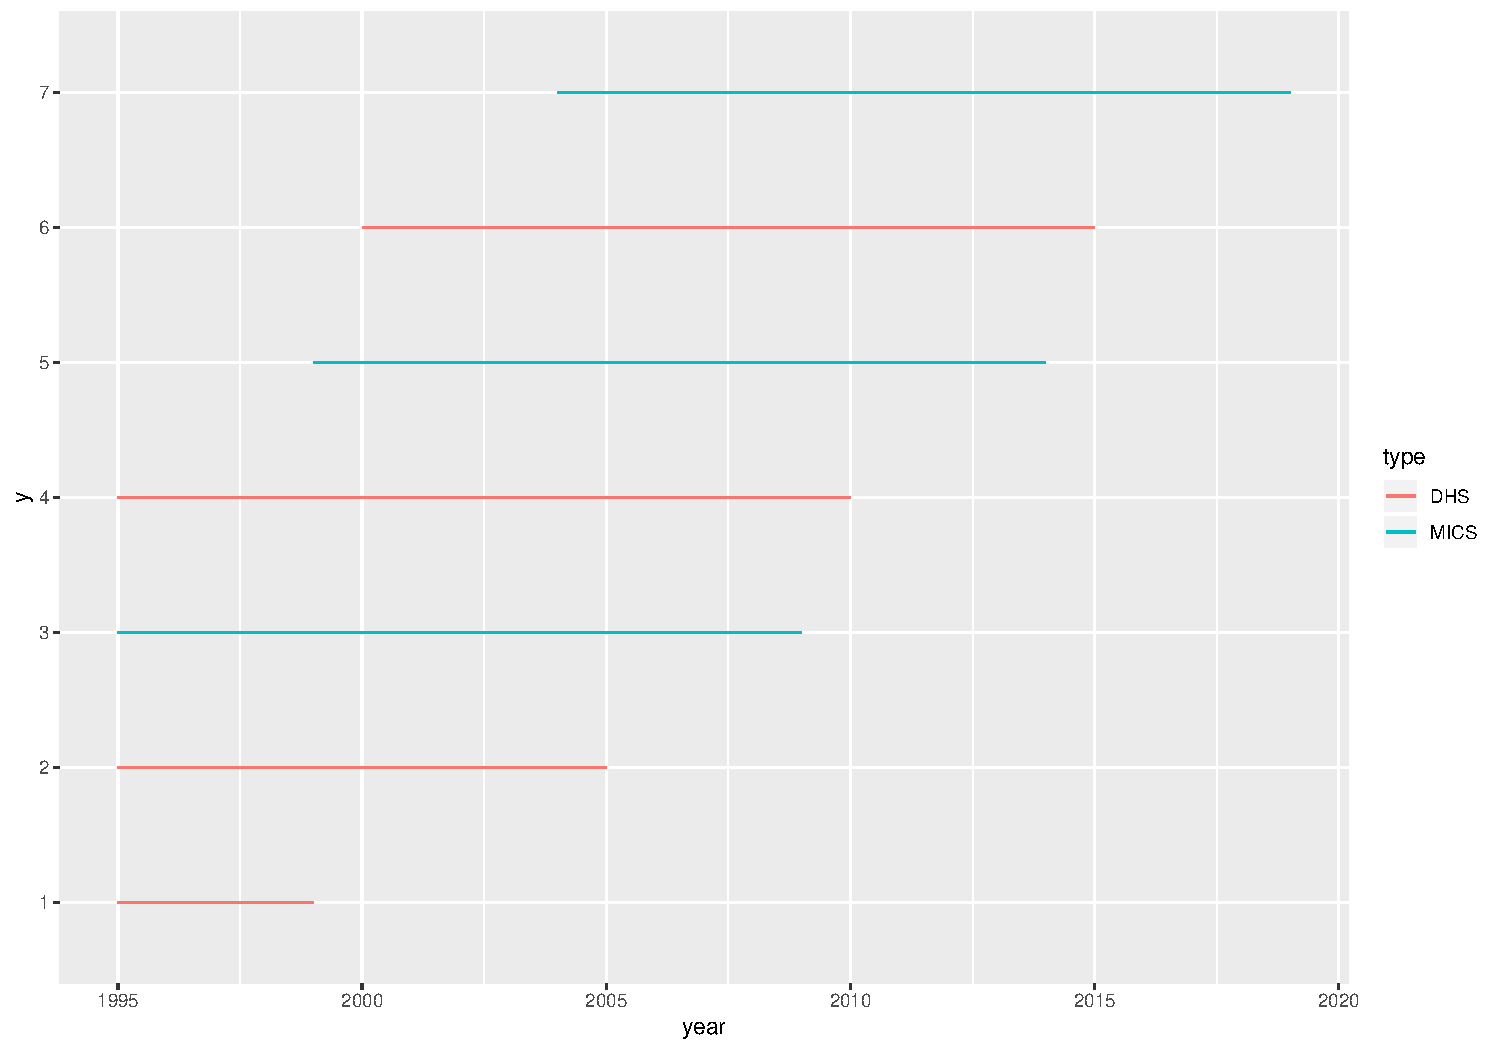
\includegraphics[height=0.8\textheight]{2020_04_UNPD_files/figure-beamer/unnamed-chunk-2-1} \end{center}

\end{frame}

\begin{frame}[t]{Data and workflow \textbar{} Non-sampling bias in
household surveys}
\protect\hypertarget{data-and-workflow-non-sampling-bias-in-household-surveys-2}{}

\begin{itemize}
\tightlist
\item
  Intersurvey analysis can estimate magnitude of bias due to overlap in
  recall periods (Masquelier, 2013; Schoumaker, 2014)
\end{itemize}

\begin{center}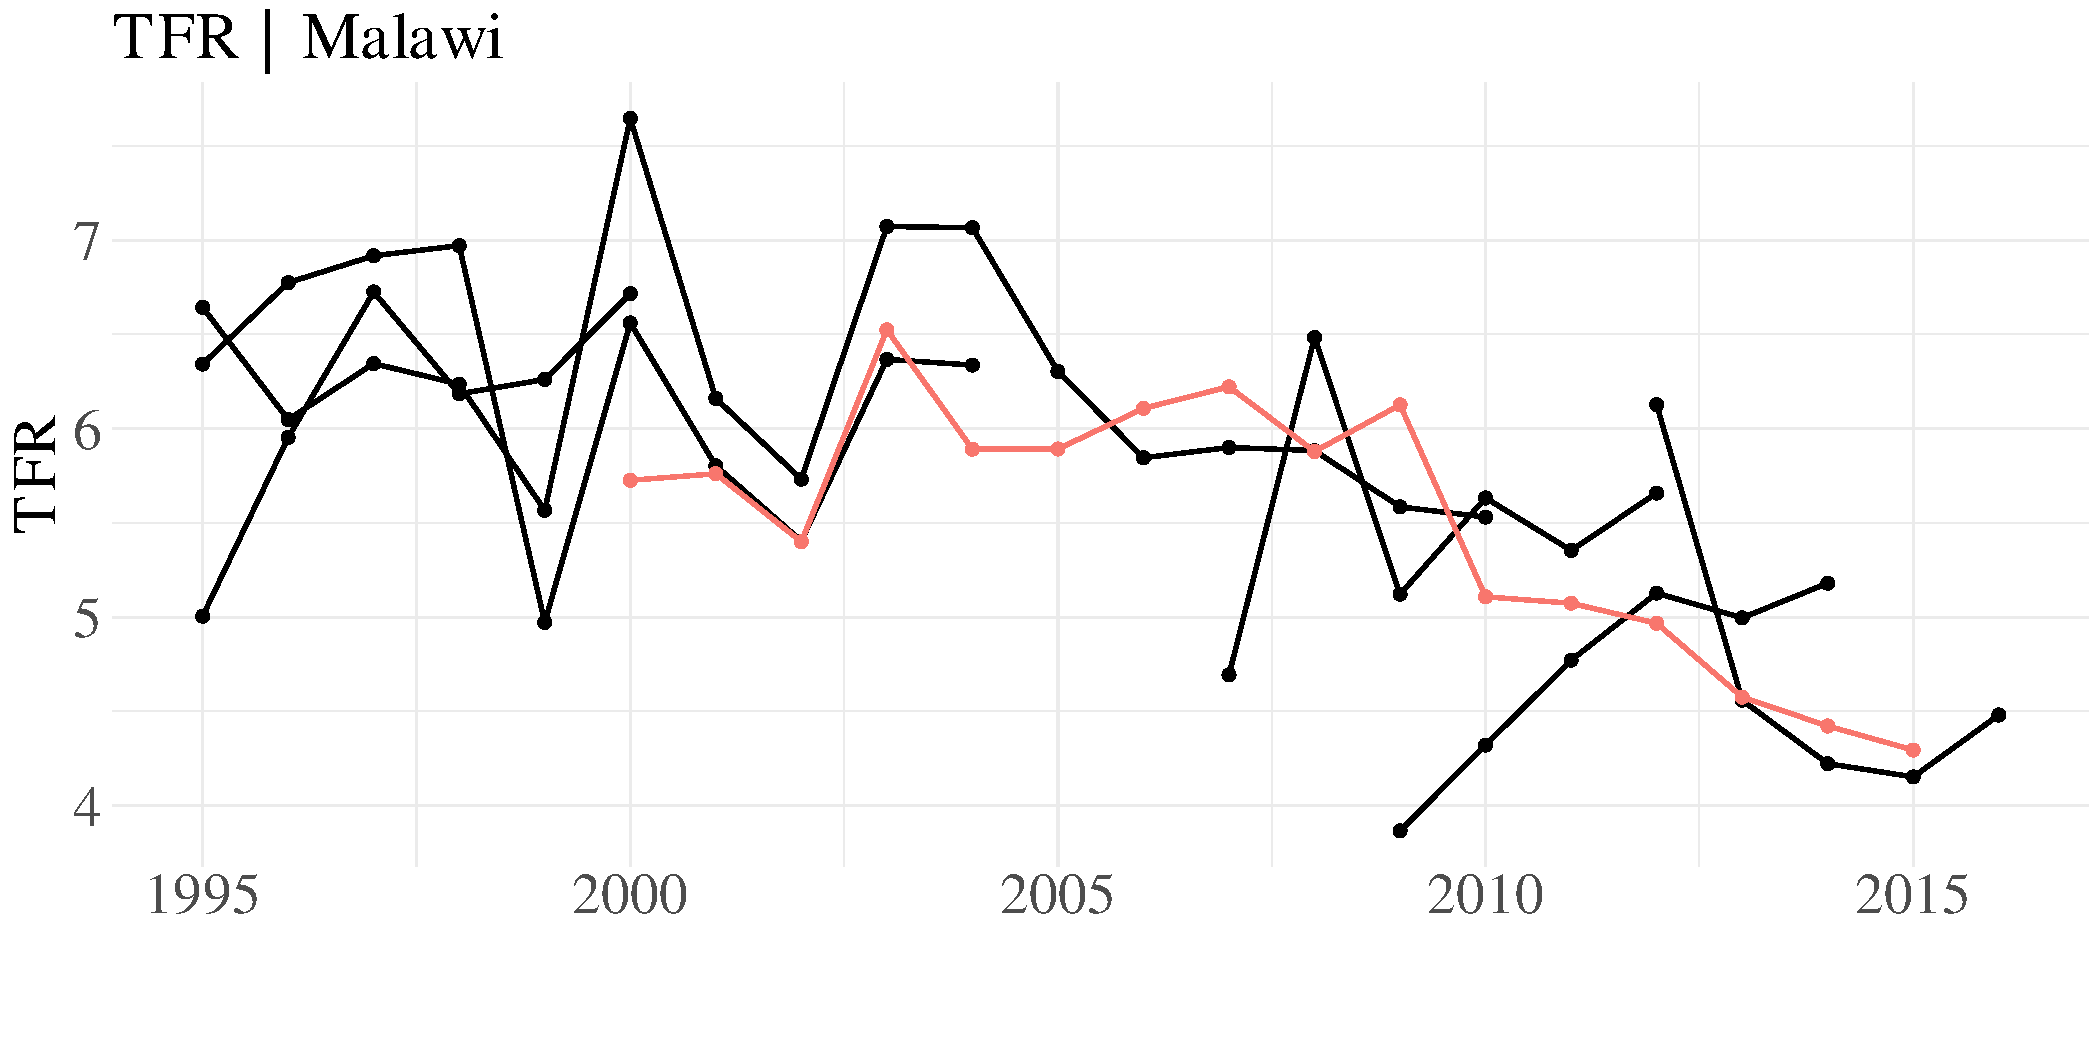
\includegraphics[height=0.65\textheight]{2020_04_UNPD_files/figure-beamer/unnamed-chunk-3-1} \end{center}

\end{frame}

\begin{frame}[t]{Data and workflow \textbar{} Non-sampling bias in
household surveys}
\protect\hypertarget{data-and-workflow-non-sampling-bias-in-household-surveys-3}{}

\begin{itemize}
\tightlist
\item
  Intersurvey analysis can estimate magnitude of bias due to overlap in
  recall periods (Masquelier, 2013; Schoumaker, 2014)
\item
  \(Y_{a,t,tips} = \mu + \alpha_a + \gamma_t + \beta_1(TIPS>5) + \omega_{tips}\)
\end{itemize}

\begin{center}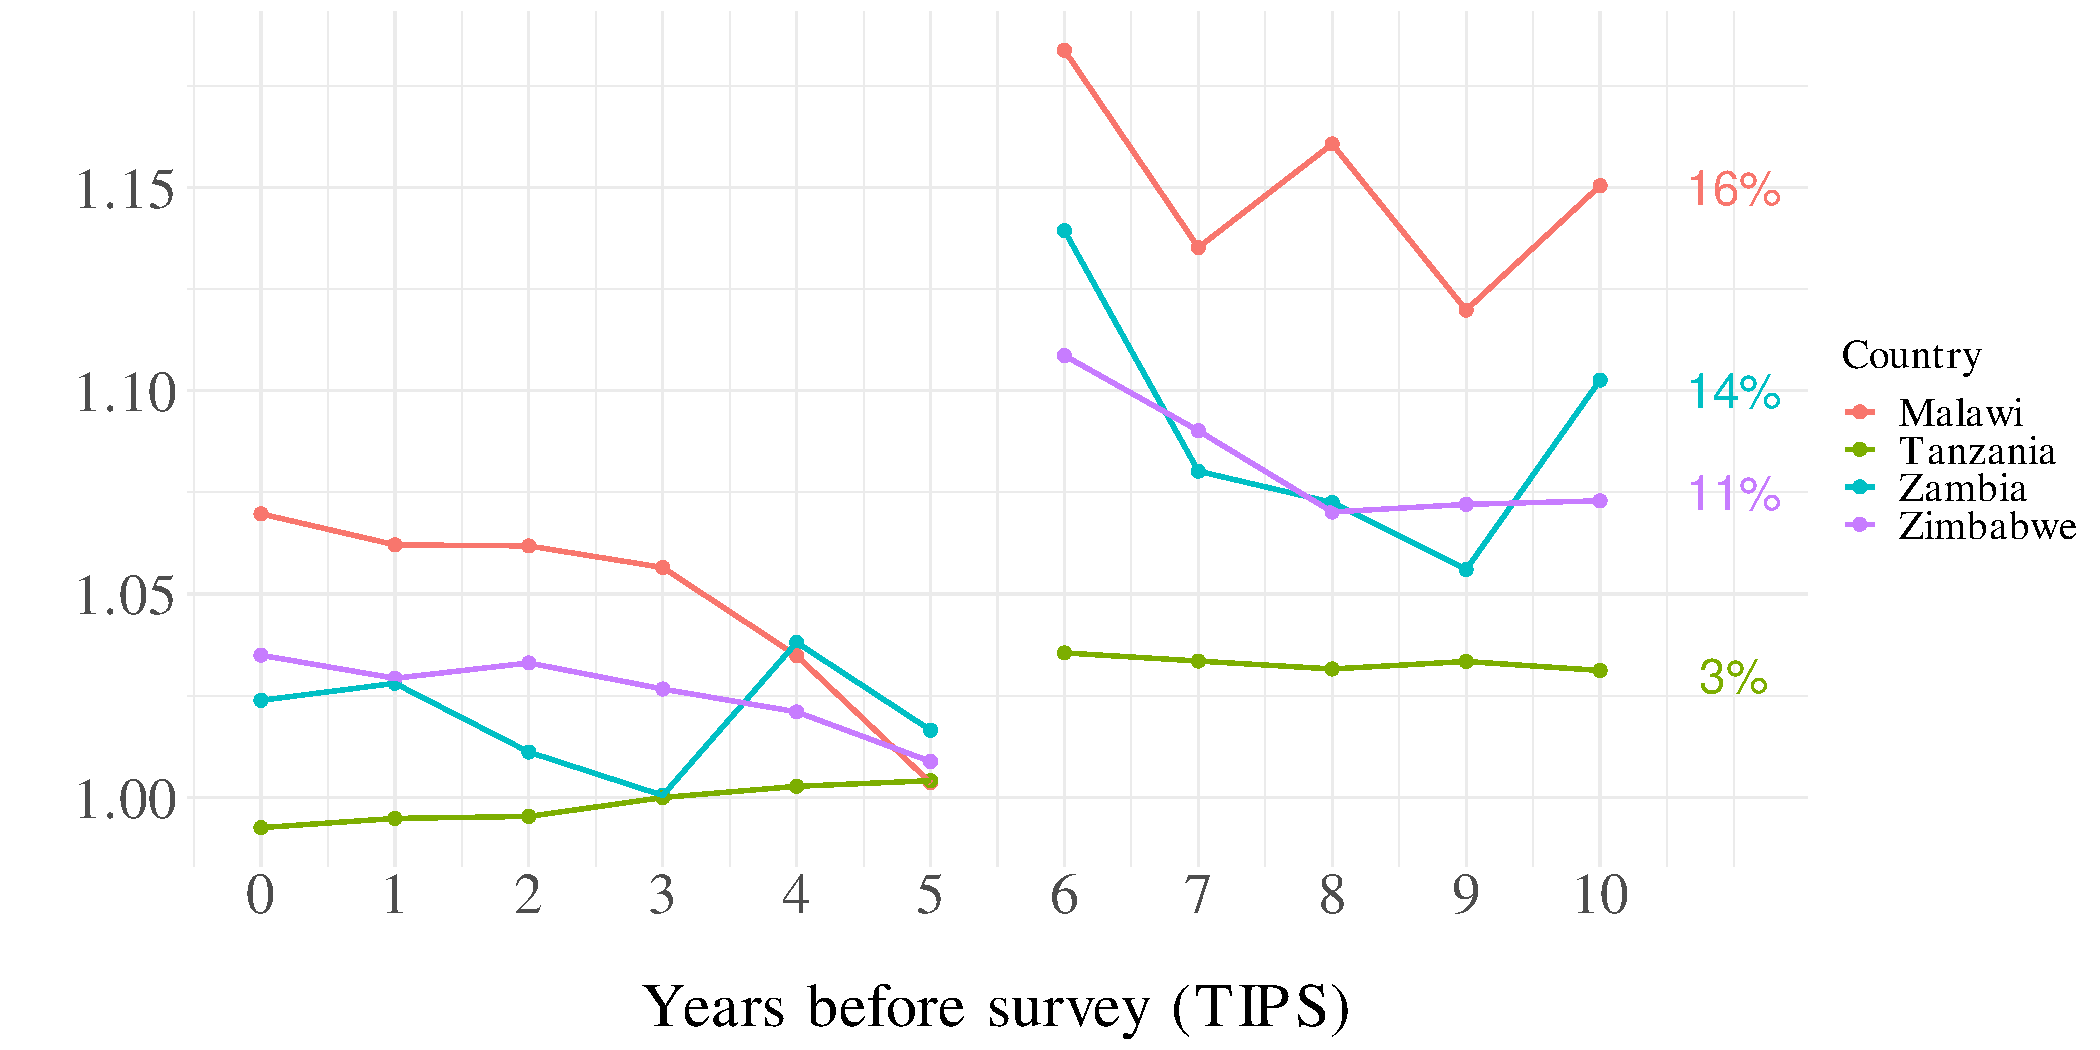
\includegraphics[height=0.5\textheight]{2020_04_UNPD_files/figure-beamer/unnamed-chunk-4-1} \end{center}

\end{frame}

\begin{frame}[t]{Model specification}
\protect\hypertarget{model-specification}{}

\[b_{ait} \sim Po( \lambda_{ait} . E_{ait} )\]
\[log(\lambda_{ait}) = \mu + \alpha_a + \gamma_t + \delta_i + \eta_{a,t} + \eta_{a,i} + \eta_{i,t}\]

Average log fertility rate: \(\mu \sim N(0, 5)\)

Age pattern: \(\alpha_a \sim RW1(\sigma^2_\alpha)\)
\(\hfill a \in \{15-19, 20-24 ... 45-49\}\)

Time trend: \(\gamma_t \sim RW2(\sigma^2_\gamma)\)
\(\hfill t \in \{1995:2020\}\)

Spatial correlation: \(\delta_i \sim BYM2(\sigma^2_\delta)\)
\(\hfill i \in \{1 ... n_i\}\)

\end{frame}

\begin{frame}[t]{Model specification}
\protect\hypertarget{model-specification-1}{}

\[b_{ait} \sim Po( \lambda_{ait} . E_{ait} )\]
\[log(\lambda_{ait}) = \mu + \alpha_a + \gamma_t + \delta_i + \eta_{a,t} + \eta_{a,i} + \eta_{i,t}\]

\(\eta_{a,t}: AR1 \otimes AR1\)

\(\eta_{a,i}: AR1 \otimes ICAR\)

\(\eta_{i,t}: ICAR \otimes AR1\)

\end{frame}

\begin{frame}[t]{Model specification}
\protect\hypertarget{model-specification-2}{}

\[b_{ait} \sim Po( \lambda_{ait} . E_{ait} )\]
\[log(\lambda_{ait}) = \mu + \alpha_a + \gamma_t + \delta_i + \eta_{a,t} + \eta_{a,i} + \eta_{i,t}\]

Observation model
\[log(\tilde{b}_{ait}) = log(\lambda_{ait} \times E_{ait}) + \beta_1 TIPS_{d} + \omega_{TIPS}\]
\(TIPS_d=\begin{cases} 0, & \text{if TIPS} < 5 \\ 1, & \text{otherwise} \end{cases}\)

\(\omega_{tips} \sim RW1(\sigma^2_\omega)\) \(\hfill tips \in \{0:14\}\)

\end{frame}

\begin{frame}{Model specification}
\protect\hypertarget{model-specification-3}{}

\[b_{ait} \sim Po( \lambda_{ait} . E_{ait} )\]
\[log(\lambda_{ait}) = \mu + \alpha_a + \gamma_t + \delta_i + \eta_{a,t} + \eta_{a,i} + \eta_{i,t}\]

Aggregation model

\[log(\tilde{b}_{at}) = \frac{\Sigma_i log(\lambda_{ait} \times E_{ait})}{E_{at}} + \beta_1 TIPS_{d} + \omega_{TIPS}\]

\end{frame}

\begin{frame}{Model specification}
\protect\hypertarget{model-specification-4}{}

\begin{itemize}
\tightlist
\item
  Model fit in Template Model Builder (TMB)
\item
  Countries take \textless{} 2 minutes to fit and sample
\end{itemize}

\end{frame}

\begin{frame}{Results}
\protect\hypertarget{results}{}

\begin{center}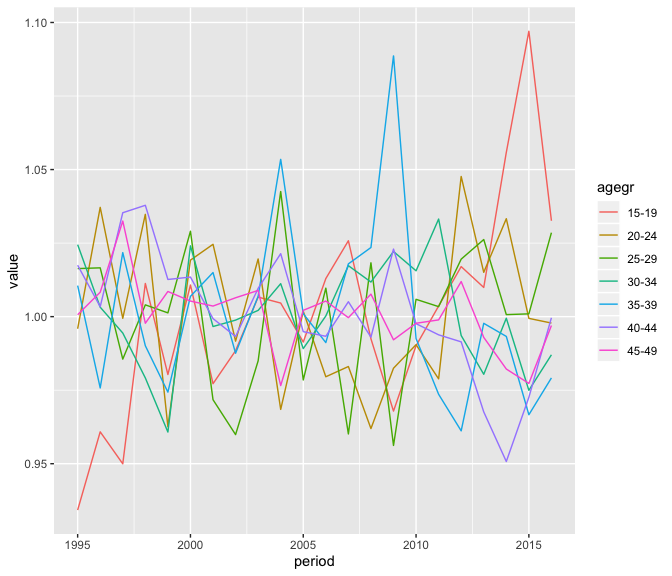
\includegraphics[height=0.9\textheight]{2020_04_UNPD_files/figure-beamer/unnamed-chunk-5-1} \end{center}

\end{frame}

\begin{frame}{Results}
\protect\hypertarget{results-1}{}

\begin{center}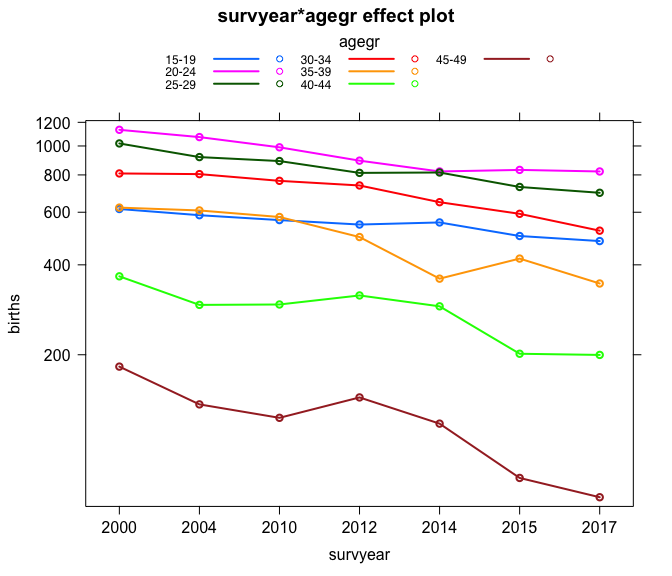
\includegraphics[height=0.9\textheight]{2020_04_UNPD_files/figure-beamer/unnamed-chunk-6-1} \end{center}

\end{frame}

\begin{frame}{Results}
\protect\hypertarget{results-2}{}

\begin{center}\includegraphics[width=1\linewidth]{2020_04_UNPD_files/figure-beamer/unnamed-chunk-7-1} \end{center}

\end{frame}

\begin{frame}{Results}
\protect\hypertarget{results-3}{}

\begin{center}\includegraphics[width=1\linewidth]{2020_04_UNPD_files/figure-beamer/unnamed-chunk-8-1} \end{center}

\end{frame}

\begin{frame}{Discussion}
\protect\hypertarget{discussion}{}

\begin{itemize}
\tightlist
\item
  There exists district-level heterogeneity that is not captured by
  admin-1 estimates
\item
  Non-sampling bias can lead to substantial distortion of fertility
  estimates in surveys

  \begin{itemize}
  \tightlist
  \item
    Role of bias adjustment depends on measure of fertility
  \end{itemize}
\item
  Can be adjusted for within automated analysis
\item
  Consideration of further non-sampling bias

  \begin{itemize}
  \tightlist
  \item
    Displacement of first birth(s) at older ages
  \end{itemize}
\end{itemize}

\end{frame}

\begin{frame}{Future work}
\protect\hypertarget{future-work}{}

\begin{itemize}
\tightlist
\item
  Structured model for fertility transition and projection (Alkema,
  2011; Sevkicova, 2012)
\item
  Survey random effects \& multi-country fitting
\item
  Census data, additional country-specific surveys, summary birth
  histories
\end{itemize}

\end{frame}

\begin{frame}{Many thanks}
\protect\hypertarget{many-thanks}{}

\textbf{Small area estimation of district-level fertility in sub-Saharan Africa}

Oli Stevens

Imperial College London

6th April 2020

\end{frame}

\begin{frame}{Extras}
\protect\hypertarget{extras}{}

\begin{figure}
\centering
\includegraphics{images/mwi tfr admin1.png}
\caption{fit}
\end{figure}

\end{frame}

\begin{frame}{Extras}
\protect\hypertarget{extras-1}{}

\begin{figure}
\centering
\includegraphics{images/nam_tfr.png}
\caption{NAM admin-1}
\end{figure}

\end{frame}

\begin{frame}{Extras}
\protect\hypertarget{extras-2}{}

\begin{figure}
\centering
\includegraphics{images/uga_tfr}
\caption{UGA admin-1}
\end{figure}

\end{frame}

\begin{frame}{Extras}
\protect\hypertarget{extras-3}{}

\begin{figure}
\centering
\includegraphics{images/zmb_tfr}
\caption{ZMB admin-1}
\end{figure}

\end{frame}

\begin{frame}{Extras}
\protect\hypertarget{extras-4}{}

\begin{center}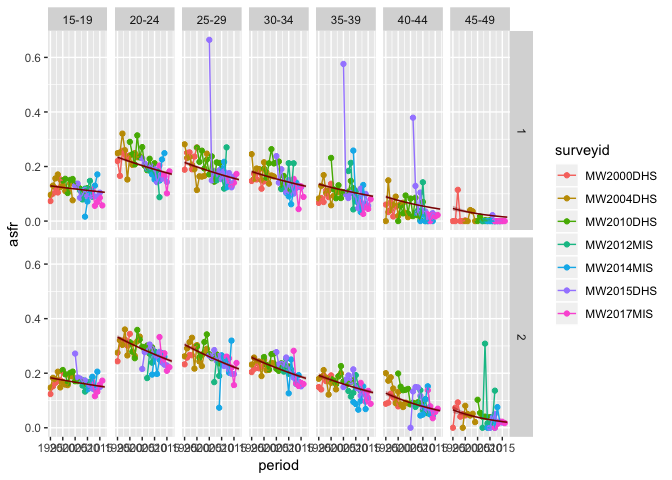
\includegraphics[width=1\linewidth]{2020_04_UNPD_files/figure-beamer/unnamed-chunk-9-1} \end{center}

\end{frame}

\end{document}
